% Author: Izaak Neutelings (September 2020)
% Inspiration: https://tex.stackexchange.com/questions/25531/adding-underbrace-in-tikz
\documentclass[border=3pt,tikz]{standalone}
\usepackage{physics}
\usepackage{ifthen}
\usepackage{tikz}
\usetikzlibrary{patterns}
\tikzset{>=latex} % for LaTeX arrow head

\colorlet{myred}{red!65!black}
\colorlet{acol}{red!50!blue!80!black!80}
\tikzstyle{ground}=[preaction={fill,top color=black!10,bottom color=black!5,shading angle=20},
                    fill,pattern=north east lines,draw=none,minimum width=0.3,minimum height=0.6]
\tikzstyle{mass}=[line width=0.6,red!30!black,fill=red!40!black!10,rounded corners=1,
                  top color=red!40!black!20,bottom color=red!40!black!10,shading angle=20]
\tikzstyle{rope}=[brown!70!black,line width=1.2,line cap=round] %very thick

% FORCES SWITCH
\tikzstyle{force}=[->,myred,thick,line cap=round]
\newcommand{\vbF}{\vb{F}}
\newboolean{showforces}
\setboolean{showforces}{true}


\begin{document}
% FRICTION static/dynamical
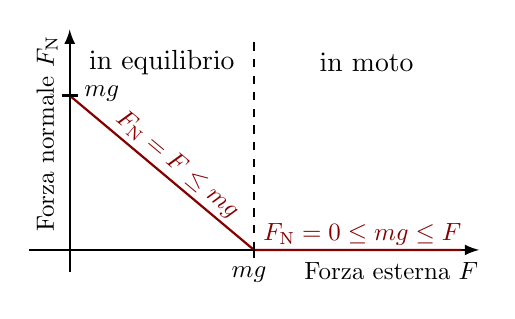
\begin{tikzpicture}
    \def\xmax{5.2}
    \def\ymax{2.8}
    \def\xc{0.45*\xmax}
    \def\yc{0.7*\ymax}
    \draw[->,thick] (-0.1*\xmax,0) -- (\xmax,0) node[right=4,below left=1, scale=0.9] {Forza esterna $F$};
    \draw[->,thick] (0,-0.1*\ymax) -- (0,\ymax) node[above left=1,rotate=90, scale=0.9] {Forza normale $F_\mathrm{N}$};
    \draw[dashed] (\xc,0) --++ (0,0.97*\ymax); % coordinate (C);
    \draw[myred!80!black,thick]
    (0,\yc) -- (\xc,0)
    node[scale=0.9,midway,right=1,above=-3,rotate={-atan2(\yc,\xc)}] {$F_\mathrm{N} = F \leq mg$}
    --++ (\xmax-1.1*\xc,0)
    node[scale=0.9,midway,right=2,above=-2] {$F_\mathrm{N} = 0 \leq mg \leq F$};
    \draw[thick] (\xc,0.1) --++ (0,-0.2) node[scale=0.9,left=2,below] {$mg$};
    \draw[thick] (-0.1,\yc) --++ (0.2,0) node[scale=0.9,above=1,right=-1] {$mg$};
    \node[] at (\xc/2,0.85*\ymax) {in equilibrio};
    \node[] at ({(\xmax+\xc)/2},0.85*\ymax) {in moto};

\end{tikzpicture}
\end{document}